\documentclass[aip,jcp,preprint,noshowkeys,superscriptaddress]{revtex4-1}
\usepackage{graphicx,dcolumn,bm,xcolor,microtype,multirow,amscd,amsmath,amssymb,amsfonts,physics,wrapfig,txfonts,setspace}
\usepackage{siunitx}[=v2]
\usepackage[version=4]{mhchem}
%\usepackage{natbib}
%\bibliographystyle{achemso}

\maxdeadcycles=200

\newcommand{\ie}{\textit{i.e.}}
\newcommand{\eg}{\textit{e.g.}}
\newcommand{\alert}[1]{\textcolor{black}{#1}}
\usepackage[normalem]{ulem}
\newcommand{\titou}[1]{\textcolor{red}{#1}}
\newcommand{\trashPFL}[1]{\textcolor{red}{\sout{#1}}}
\newcommand{\PFL}[1]{\titou{(\underline{\bf PFL}: #1)}}
\newcommand{\toto}[1]{\textcolor{green}{#1}}
\newcommand{\trashAS}[1]{\textcolor{green}{\sout{#1}}}
\newcommand{\AS}[1]{\toto{(\underline{\bf AS}: #1)}}
\newcommand{\ant}[1]{\textcolor{orange}{#1}}
\newcommand{\SupInf}{\textcolor{blue}{Supporting Information}}

\newcommand{\mc}{\multicolumn}
\newcommand{\fnm}{\footnotemark}
\newcommand{\fnt}{\footnotetext}
\newcommand{\tabc}[1]{\multicolumn{1}{c}{#1}}
\newcommand{\QP}{\textsc{quantum package}}

\newcommand{\EHF}{E_\text{HF}}
\newcommand{\EDOCI}{E_\text{DOCI}}
\newcommand{\EFCI}{E_\text{FCI}}

\renewcommand{\thesection}{S\arabic{section}}
\renewcommand{\thetable}{S\arabic{table}}
\renewcommand{\thefigure}{S\arabic{figure}}
\renewcommand{\theequation}{S\arabic{equation}}

\usepackage[
	colorlinks=true,
    citecolor=blue,
    breaklinks=true
	]{hyperref}
\urlstyle{same}

\begin{document}

\newcommand{\LCPQ}{Laboratoire de Chimie et Physique Quantiques (UMR 5626), Universit\'e de Toulouse, CNRS, UPS, France}

\title{Supporting Information for ``Seniority and hierarchy configuration interaction for radicals and excited states''}

\author{F\'abris Kossoski}
\email{fkossoski@irsamc.ups-tlse.fr}
\affiliation{\LCPQ}
\author{Pierre-Fran\c{c}ois Loos}
\email{loos@irsamc.ups-tlse.fr}
\affiliation{\LCPQ}

% Abstract
\begin{abstract}
%Here comes the abstract.
%\bigskip
%\begin{center}
%        \boxed{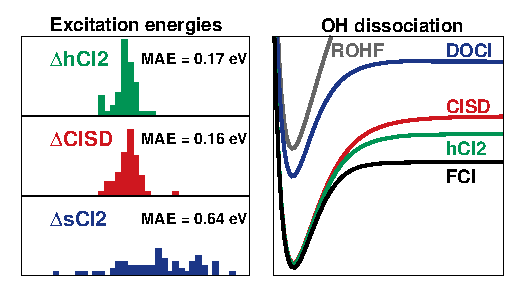
\includegraphics[width=0.4\linewidth]{TOC}}
%\end{center}
%\bigskip
\end{abstract}

% Title
\maketitle

%%%%%%%%%%%%%%%%%%%%%%%%%%%%%%%%%%%%%%%%%%%%%%%%%%
%\section{Equilibrium geometry of ethylene}
%\label{sec:ethylene}
%%%%%%%%%%%%%%%%%%%%%%%%%%%%%%%%%%%%%%%%%%%%%%%%%%

Equilibrium geometry of ethylene, in atomic units, obtained from Ref. \onlinecite{Loos_2018}:
\begin{singlespace}
\begin{verbatim}
C    0.00000000       1.26026583        0.00000000 
C    0.00000000      -1.26026583        0.00000000 
H    0.00000000       2.32345976        1.74287672 
H    0.00000000      -2.32345976        1.74287672 
H    0.00000000       2.32345976       -1.74287672 
H    0.00000000      -2.32345976       -1.74287672 
\end{verbatim}
\end{singlespace}

Equilibrium geometry of vinyl, in atomic units, obtained from Ref. \onlinecite{Loos_2020}:
\begin{singlespace}
\begin{verbatim}
C    0.00000000       1.16769663       -0.04303146
C    0.00000000      -1.29945364        0.15810072
H    0.00000000       2.38429609        1.59801822
H    0.00000000       2.08759130       -1.87998309
H    0.00000000      -2.90307925       -1.08814513
\end{verbatim}
\end{singlespace}

%%%%%%%%%%%%%%%%%%%%%%%%%%%%%%%%%%%%%%%%%%%%%%%%%%
%\section{\ce{Computational details}}
%\label{sec:comp_details}
%%%%%%%%%%%%%%%%%%%%%%%%%%%%%%%%%%%%%%%%%%%%%%%%%%

By fitting the computed potential energy curves with a Morse potential, we obtained harmonic vibrational frequencies and equilibrium geometries.
The following intervals have been considered for the fitting:
\begin{itemize}
\item \ce{HF}: \SI{0.8}{\angstrom} to \SI{1.3}{\angstrom}
\item \ce{F2}: \SI{1.25}{\angstrom} to \SI{1.65}{\angstrom}
\item ethylene: \SI{2.2}{\bohr} to \SI{2.9}{\bohr}
\item \ce{N2}: \SI{0.95}{\angstrom} to \SI{1.3}{\angstrom}
\item \ce{H4}: \SI{1.45}{\bohr} to \SI{1.95}{\bohr}
\item \ce{H8}: \SI{1.6}{\bohr} to \SI{2.05}{\bohr}
\item \ce{OH}: \SI{0.85}{\angstrom} to \SI{1.2}{\angstrom}
\item \ce{CN}: \SI{1.0}{\angstrom} to \SI{1.4}{\angstrom}
\item vinyl: \SI{2.35}{\bohr} to \SI{2.7}{\bohr}
\item \ce{H7}: \SI{1.6}{\bohr} to \SI{2.05}{\bohr}
\end{itemize}

The non-parallelity error and distance error were computed for the following intervals:
\begin{itemize}
\item \ce{HF}: \SI{0.5}{\angstrom} to \SI{6}{\angstrom}
\item \ce{F2}: \SI{0.95}{\angstrom} to \SI{8}{\angstrom}
\item ethylene: \SI{1.5}{\bohr} to \SI{16}{\bohr}
\item \ce{N2}: \SI{0.7}{\angstrom} to \SI{4}{\angstrom}
\item \ce{H4}: \SI{1}{\bohr} to \SI{10}{\bohr}
\item \ce{H8}: \SI{1}{\bohr} to \SI{10}{\bohr}
\item \ce{OH}: \SI{0.6}{\angstrom} to \SI{8}{\angstrom}
\item \ce{CN}: \SI{0.7}{\angstrom} to \SI{4}{\angstrom}
\item vinyl: \SI{1.7}{\bohr} to \SI{9}{\bohr}
\item \ce{H7}: \SI{1}{\bohr} to \SI{10}{\bohr}
\end{itemize}


\clearpage


%%% FIG S1 %%%
\begin{figure*}%[h!]
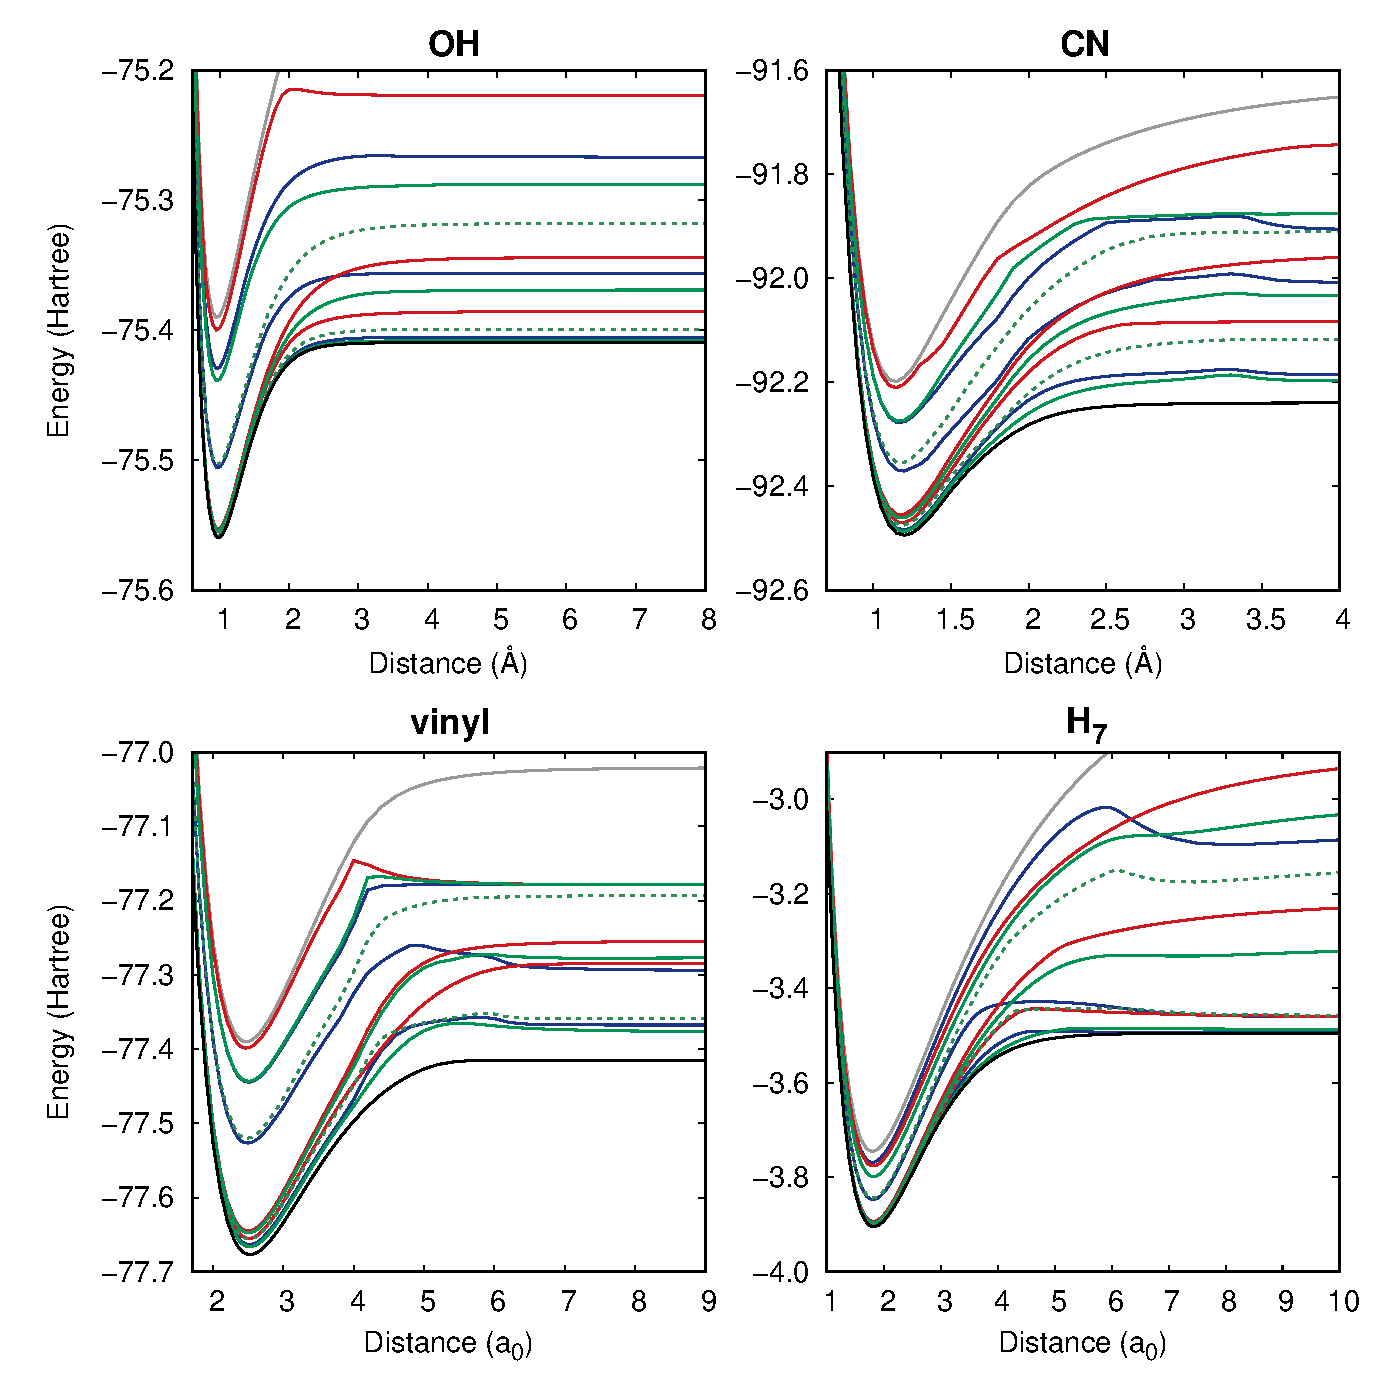
\includegraphics[width=1.0\linewidth]{plot_pes}
\caption{
Potential energy curves for \ce{OH}, \ce{CN}, vinyl, and \ce{H7},
according to hCI (green), excitation-based CI (red) and sCI (blue) models.
}
\label{fig:plot_pes}
\end{figure*}
%%% %%% %%%


%%% FIG S3 %%%
\begin{figure*}%[h!]
\includegraphics[width=1.0\linewidth]{plot_pes_closed}
\caption{
Potential energy curves for \ce{HF}, \ce{F2}, \ce{N2}, ethylene, \ce{H4}, and \ce{H8},
according to hCI (green), excitation-based CI (red) and sCI (blue) models,
with (light tones) and without (dark tones) the EN2 perturbative correction.
Results first reported in Ref. \onlinecite{Kossoski_2022}.
}
\label{fig:plot_pes_closed}
\end{figure*}
%%% %%% %%%

%%% FIG S3 %%%
\begin{figure*}%[h!]
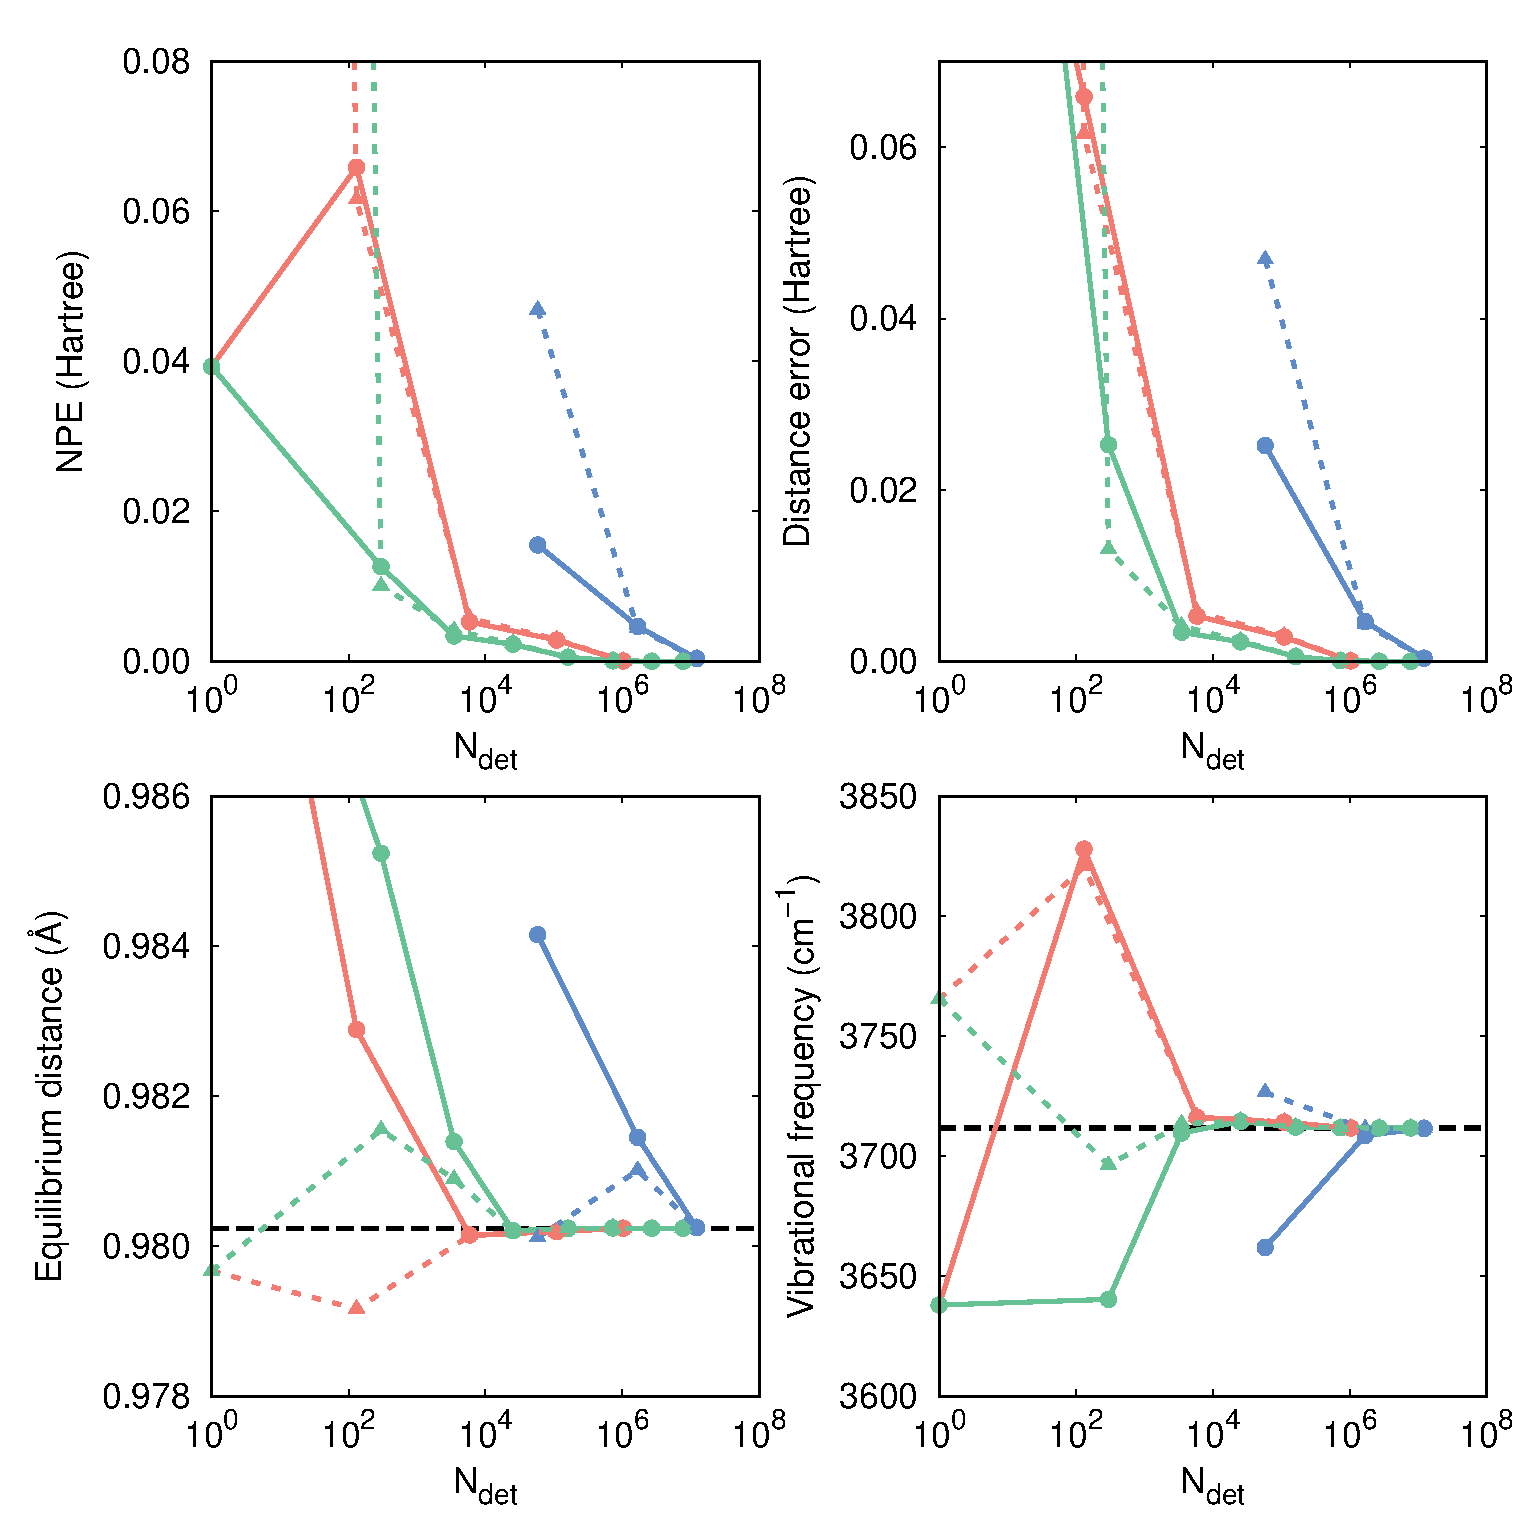
\includegraphics[width=1.0\linewidth]{plot_pt2_rpt2_OH}
\caption{
\ce{OH}
}
\label{fig:plot_pt2_rpt2_oh}
\end{figure*}
%%% %%% %%%

%%% FIG S3 %%%
\begin{figure*}%[h!]
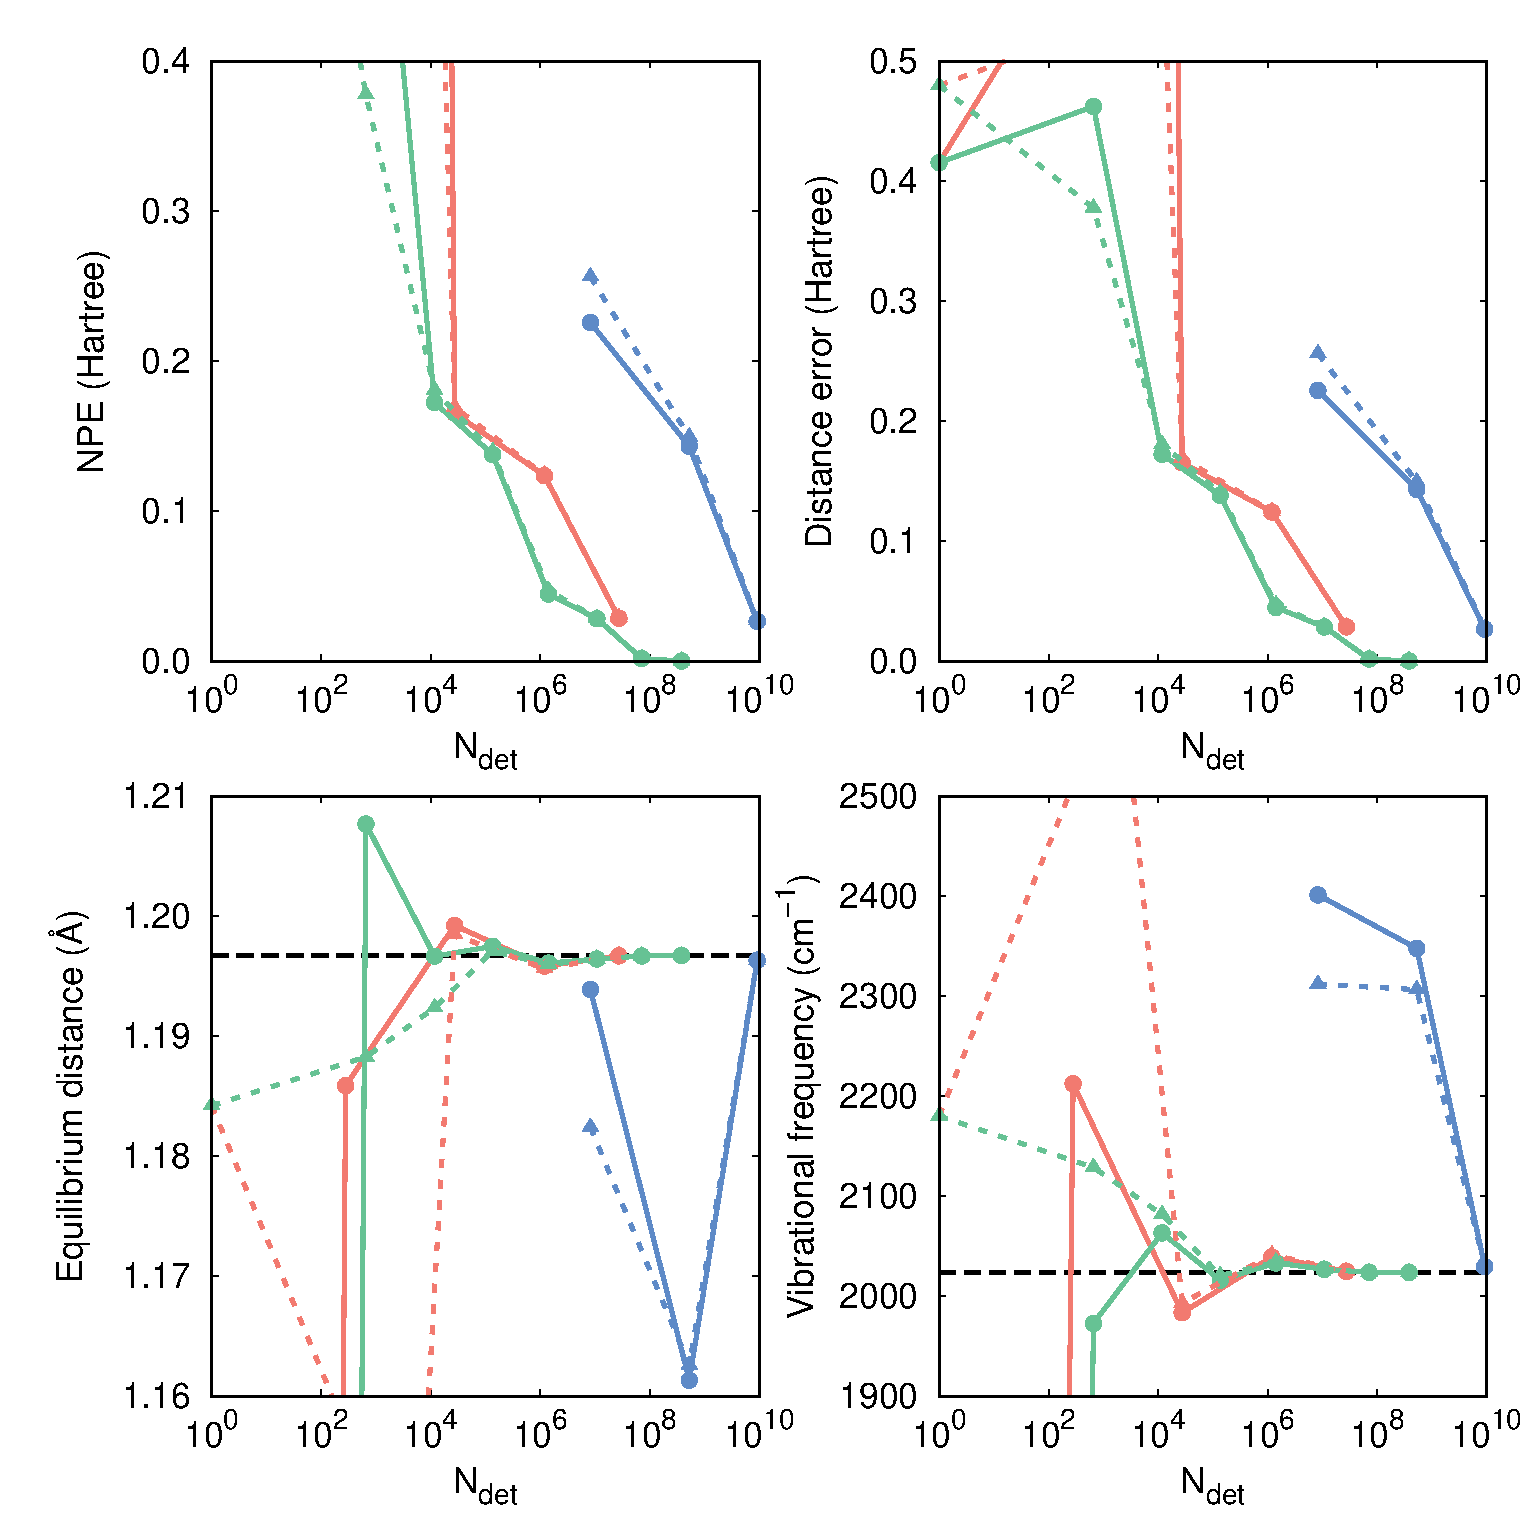
\includegraphics[width=1.0\linewidth]{plot_pt2_rpt2_CN}
\caption{
\ce{CN}
}
\label{fig:plot_pt2_rpt2_cn}
\end{figure*}
%%% %%% %%%

%%% FIG S3 %%%
\begin{figure*}%[h!]
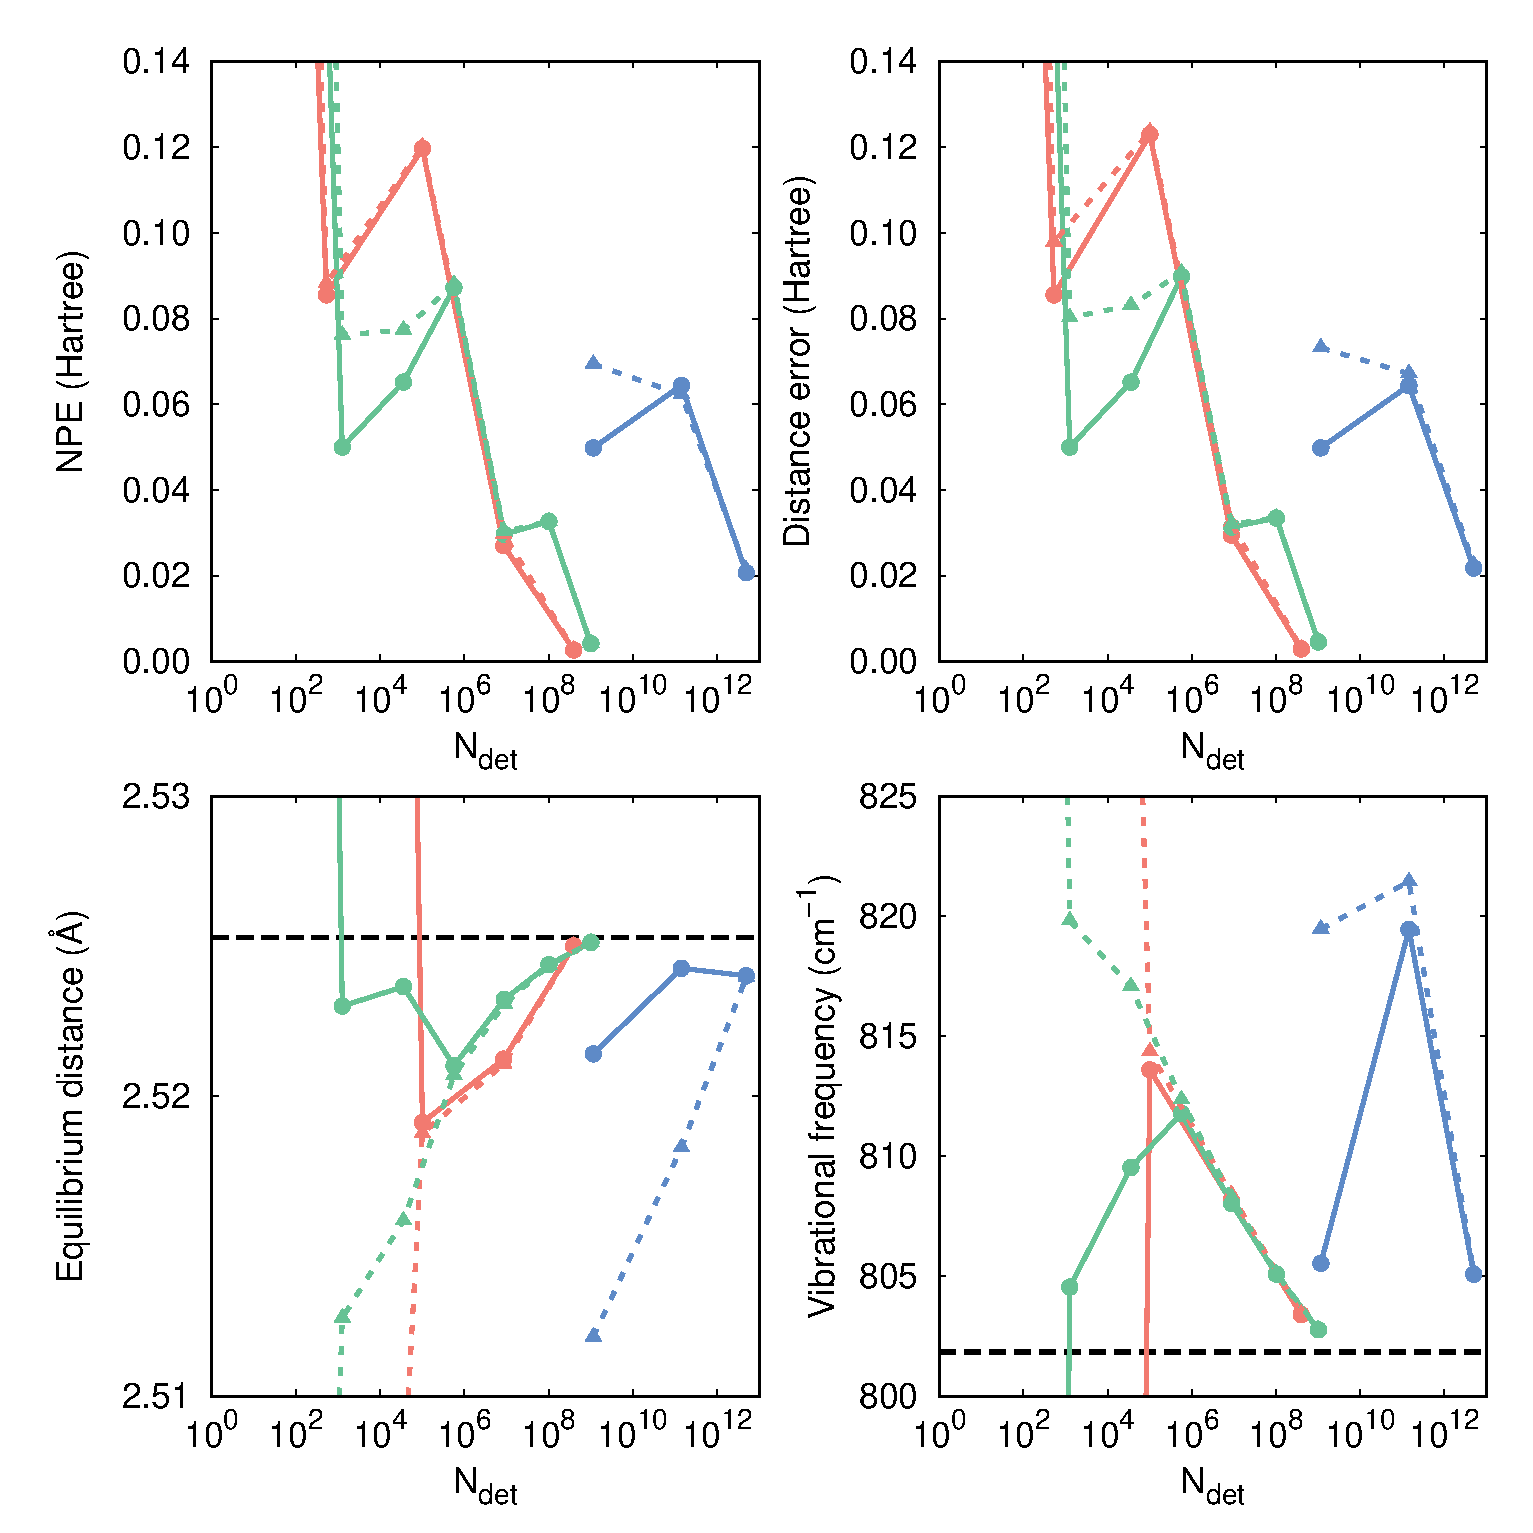
\includegraphics[width=1.0\linewidth]{plot_pt2_rpt2_vinyl}
\caption{
vinyl
}
\label{fig:plot_pt2_rpt2_vinyl}
\end{figure*}
%%% %%% %%%

%%% FIG S3 %%%
\begin{figure*}%[h!]
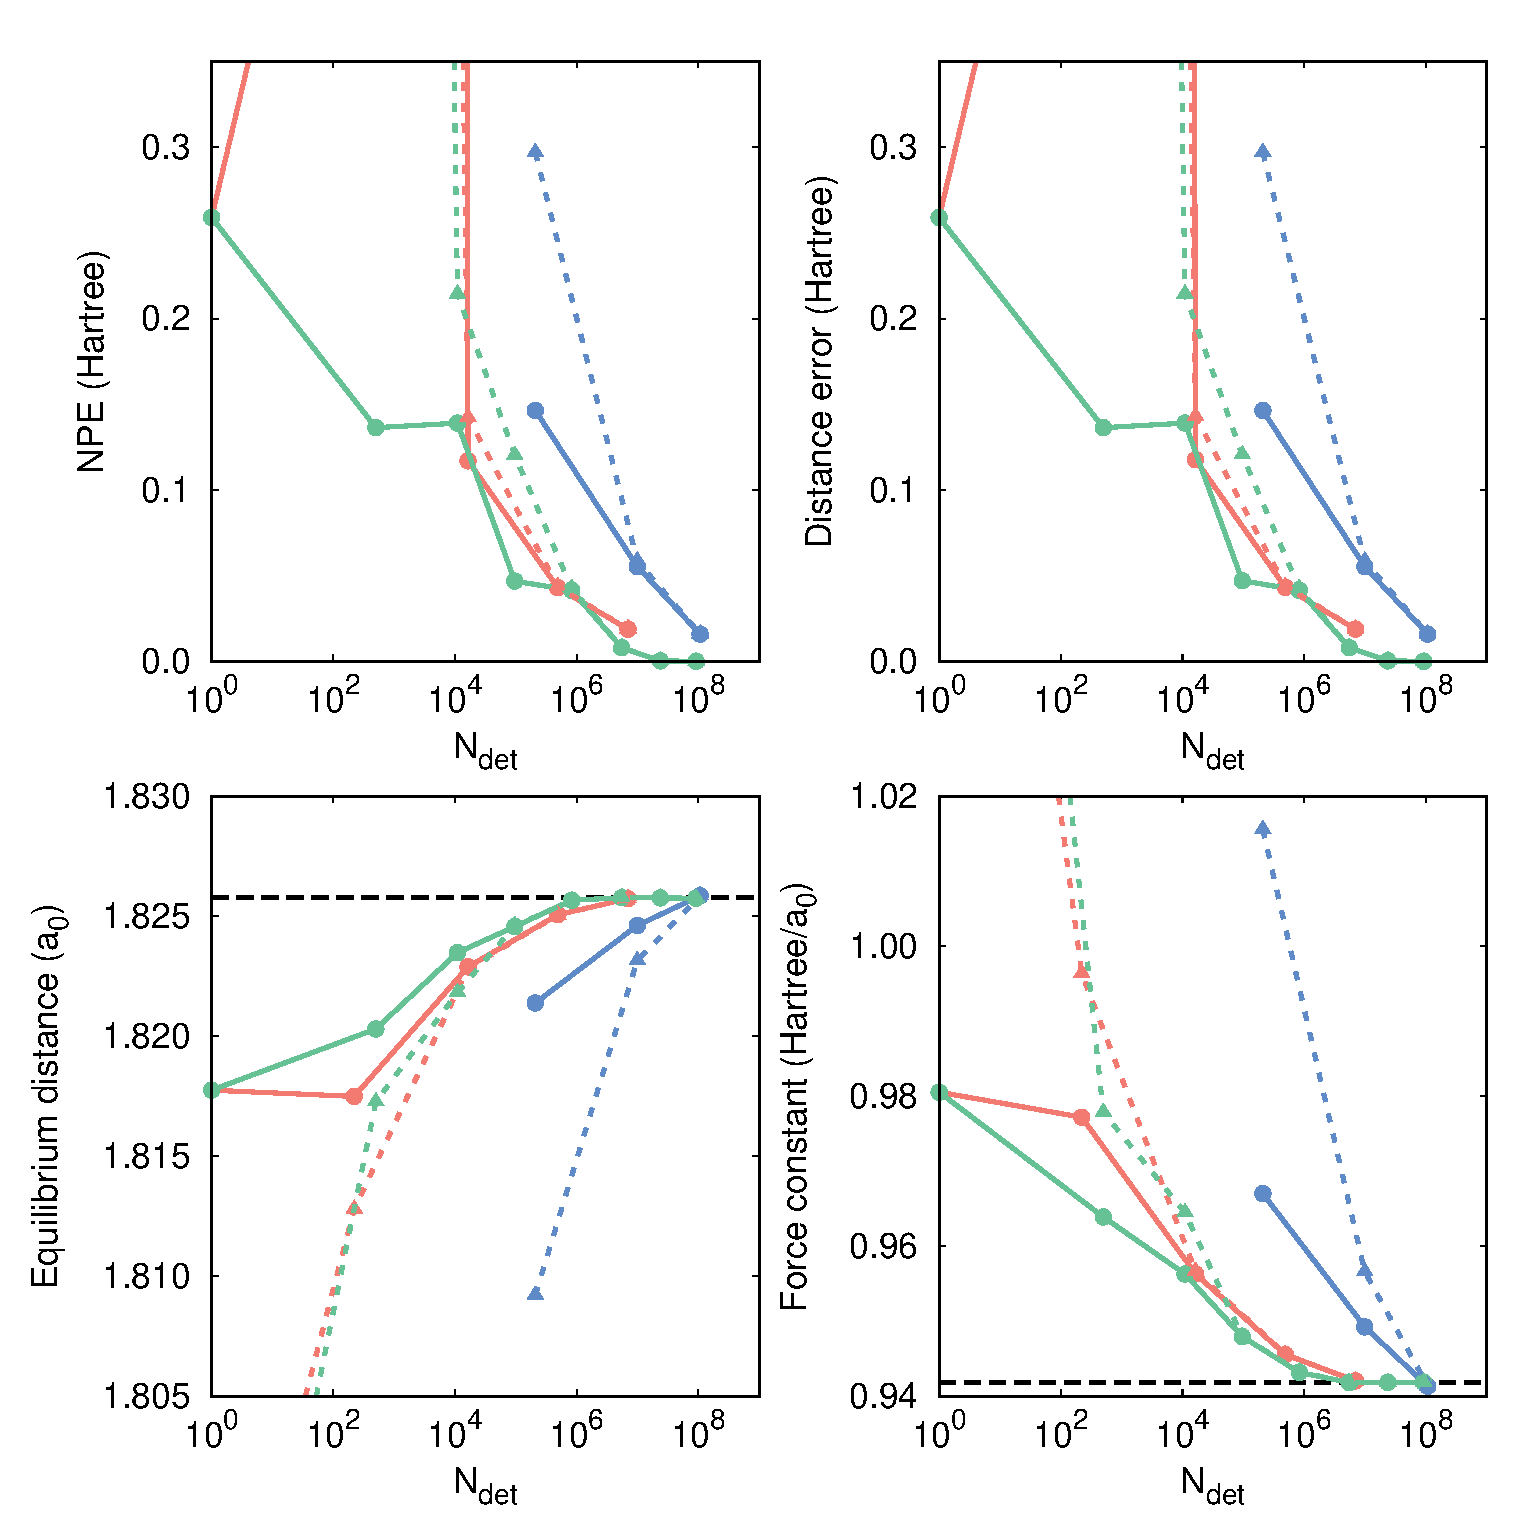
\includegraphics[width=1.0\linewidth]{plot_pt2_rpt2_H7}
\caption{
\ce{H7}
}
\label{fig:plot_pt2_rpt2_h7}
\end{figure*}
%%% %%% %%%

%%% FIG S3 %%%
\begin{figure*}%[h!]
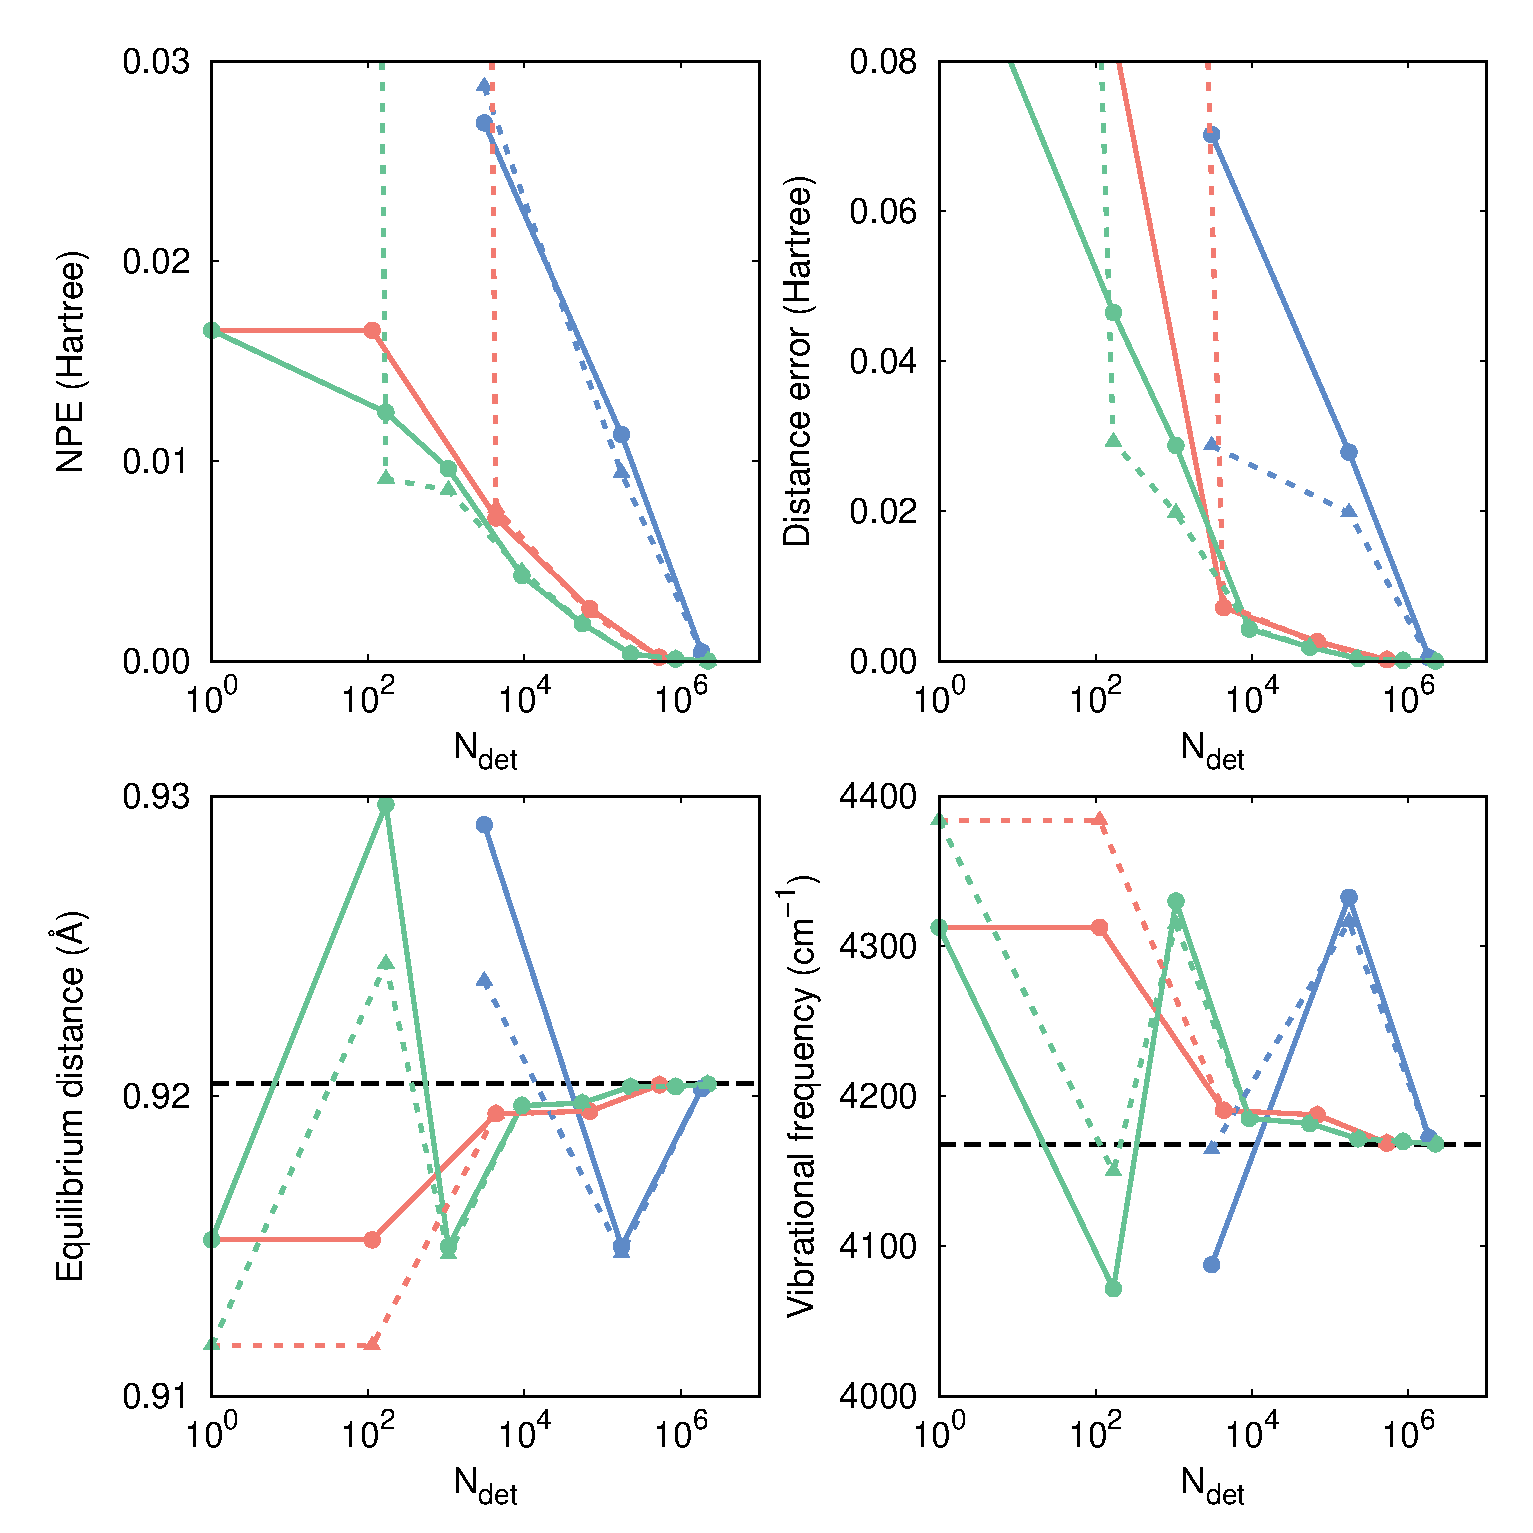
\includegraphics[width=1.0\linewidth]{plot_pt2_rpt2_HF}
\caption{
\ce{HF}
}
\label{fig:plot_pt2_rpt2_hf}
\end{figure*}
%%% %%% %%%

%%% FIG S3 %%%
\begin{figure*}%[h!]
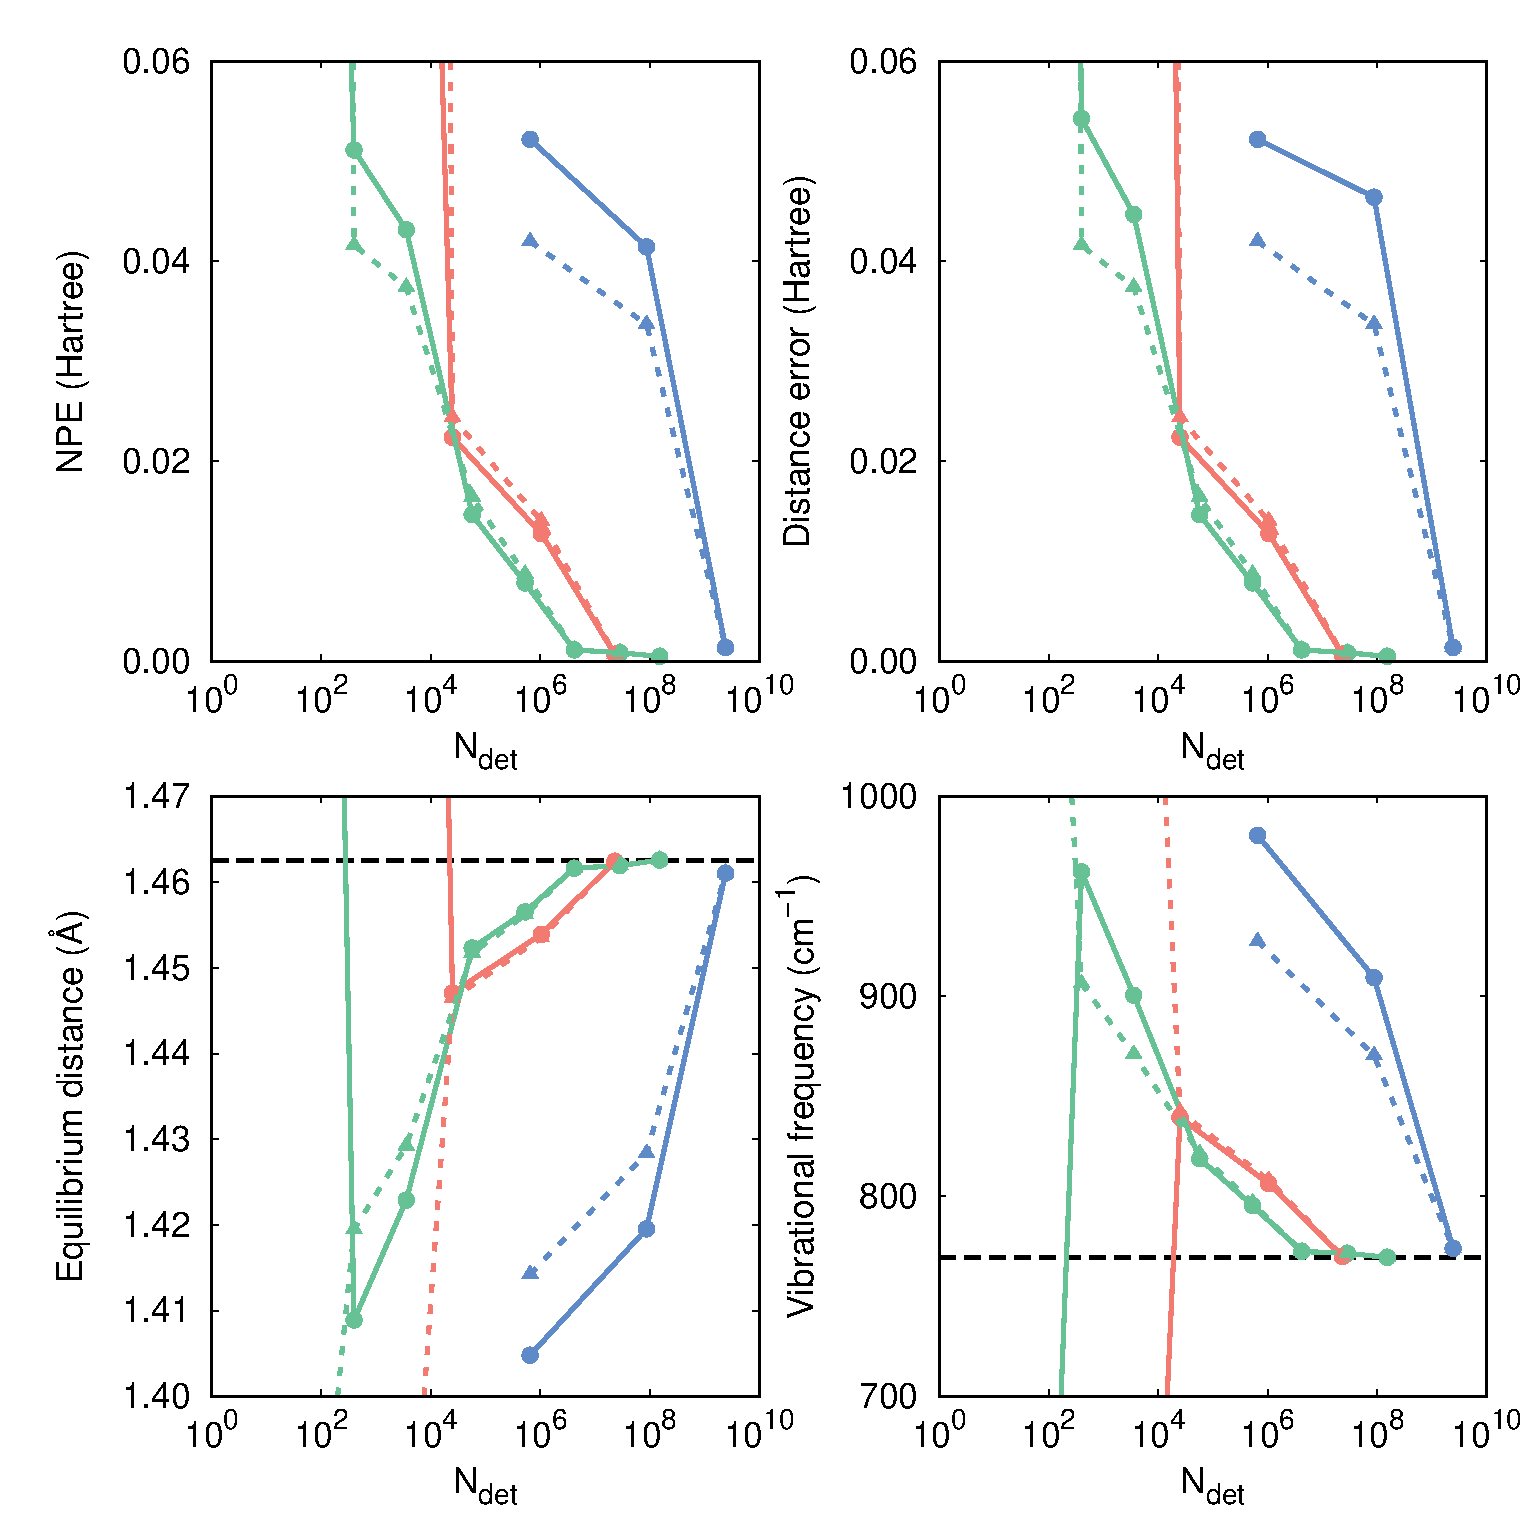
\includegraphics[width=1.0\linewidth]{plot_pt2_rpt2_F2}
\caption{
\ce{F2}
}
\label{fig:plot_pt2_rpt2_f2}
\end{figure*}
%%% %%% %%%

%%% FIG S3 %%%
\begin{figure*}%[h!]
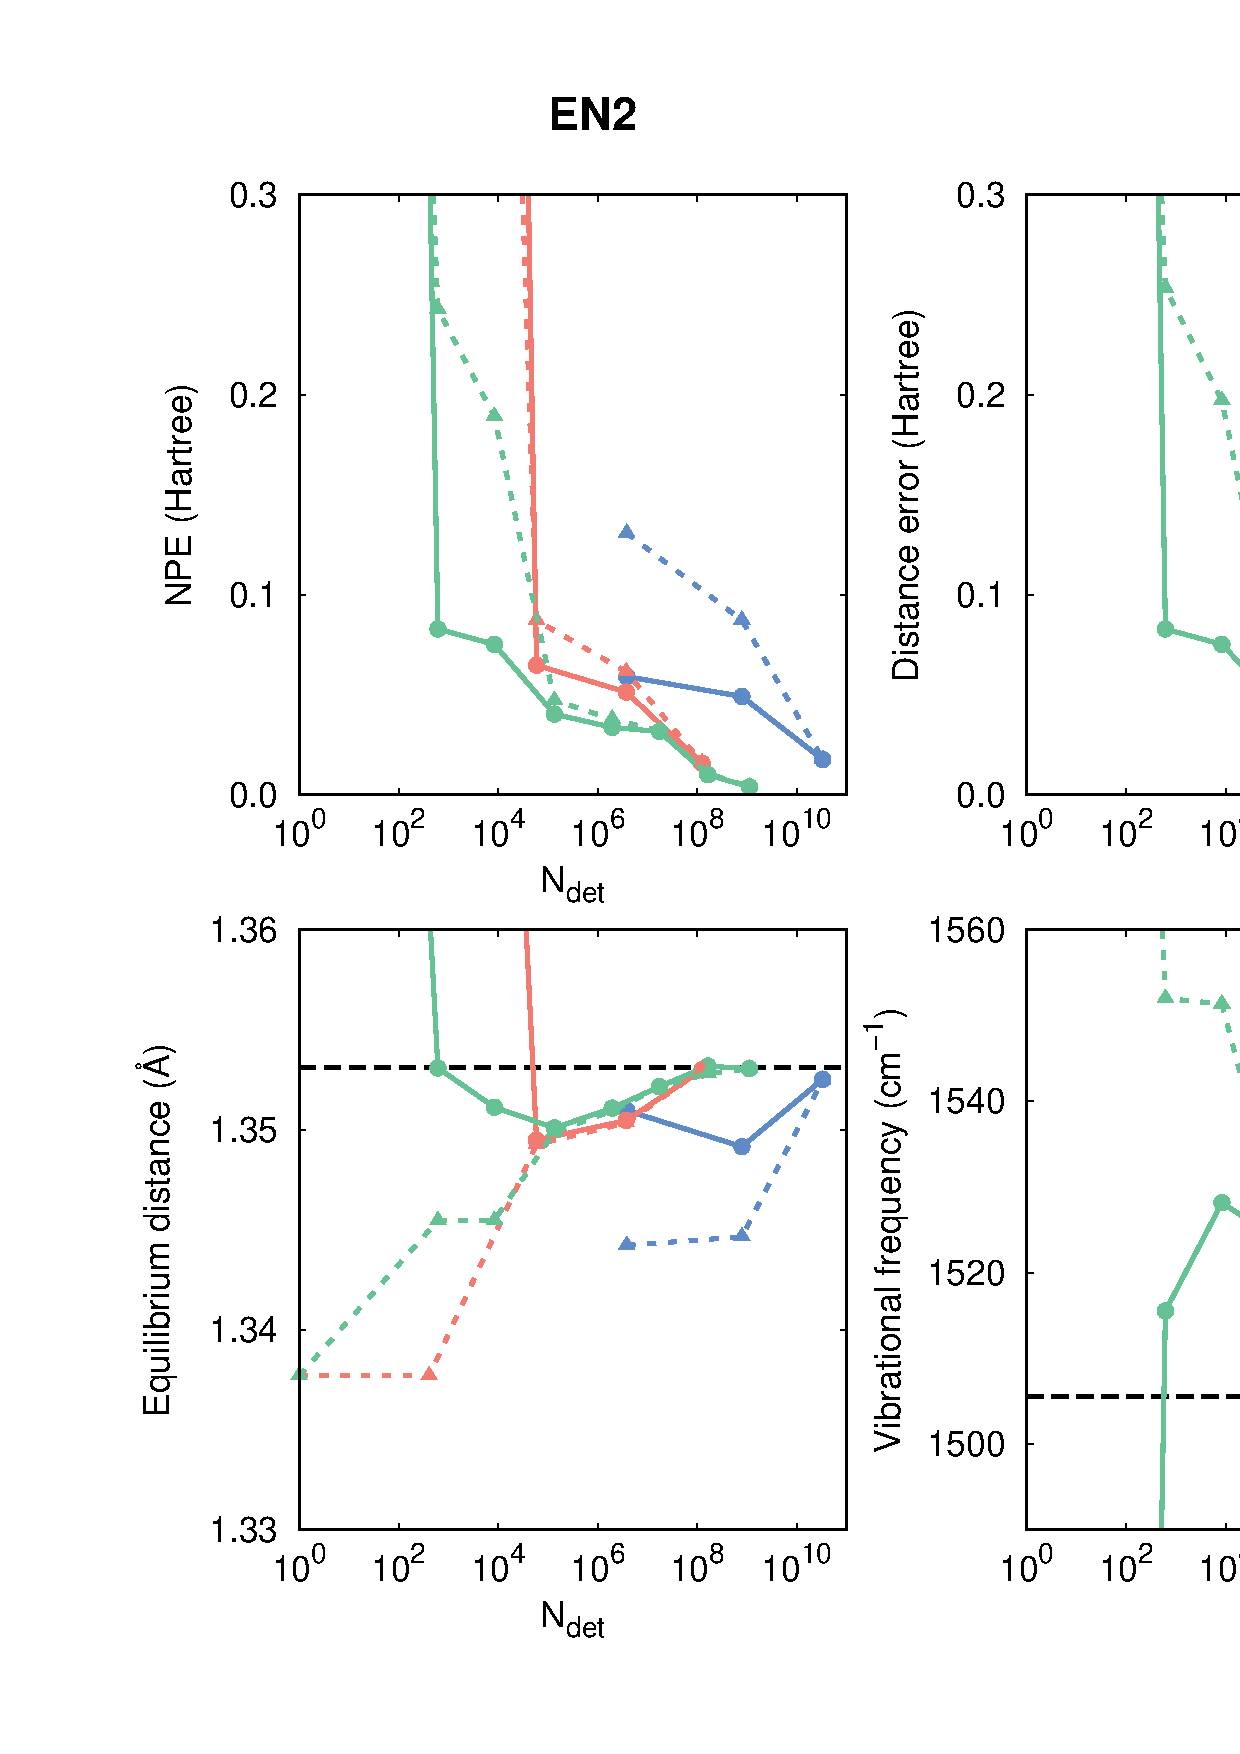
\includegraphics[width=1.0\linewidth]{plot_pt2_rpt2_ethylene}
\caption{
ethylene
}
\label{fig:plot_pt2_rpt2_ethylene}
\end{figure*}
%%% %%% %%%

%%% FIG S3 %%%
\begin{figure*}%[h!]
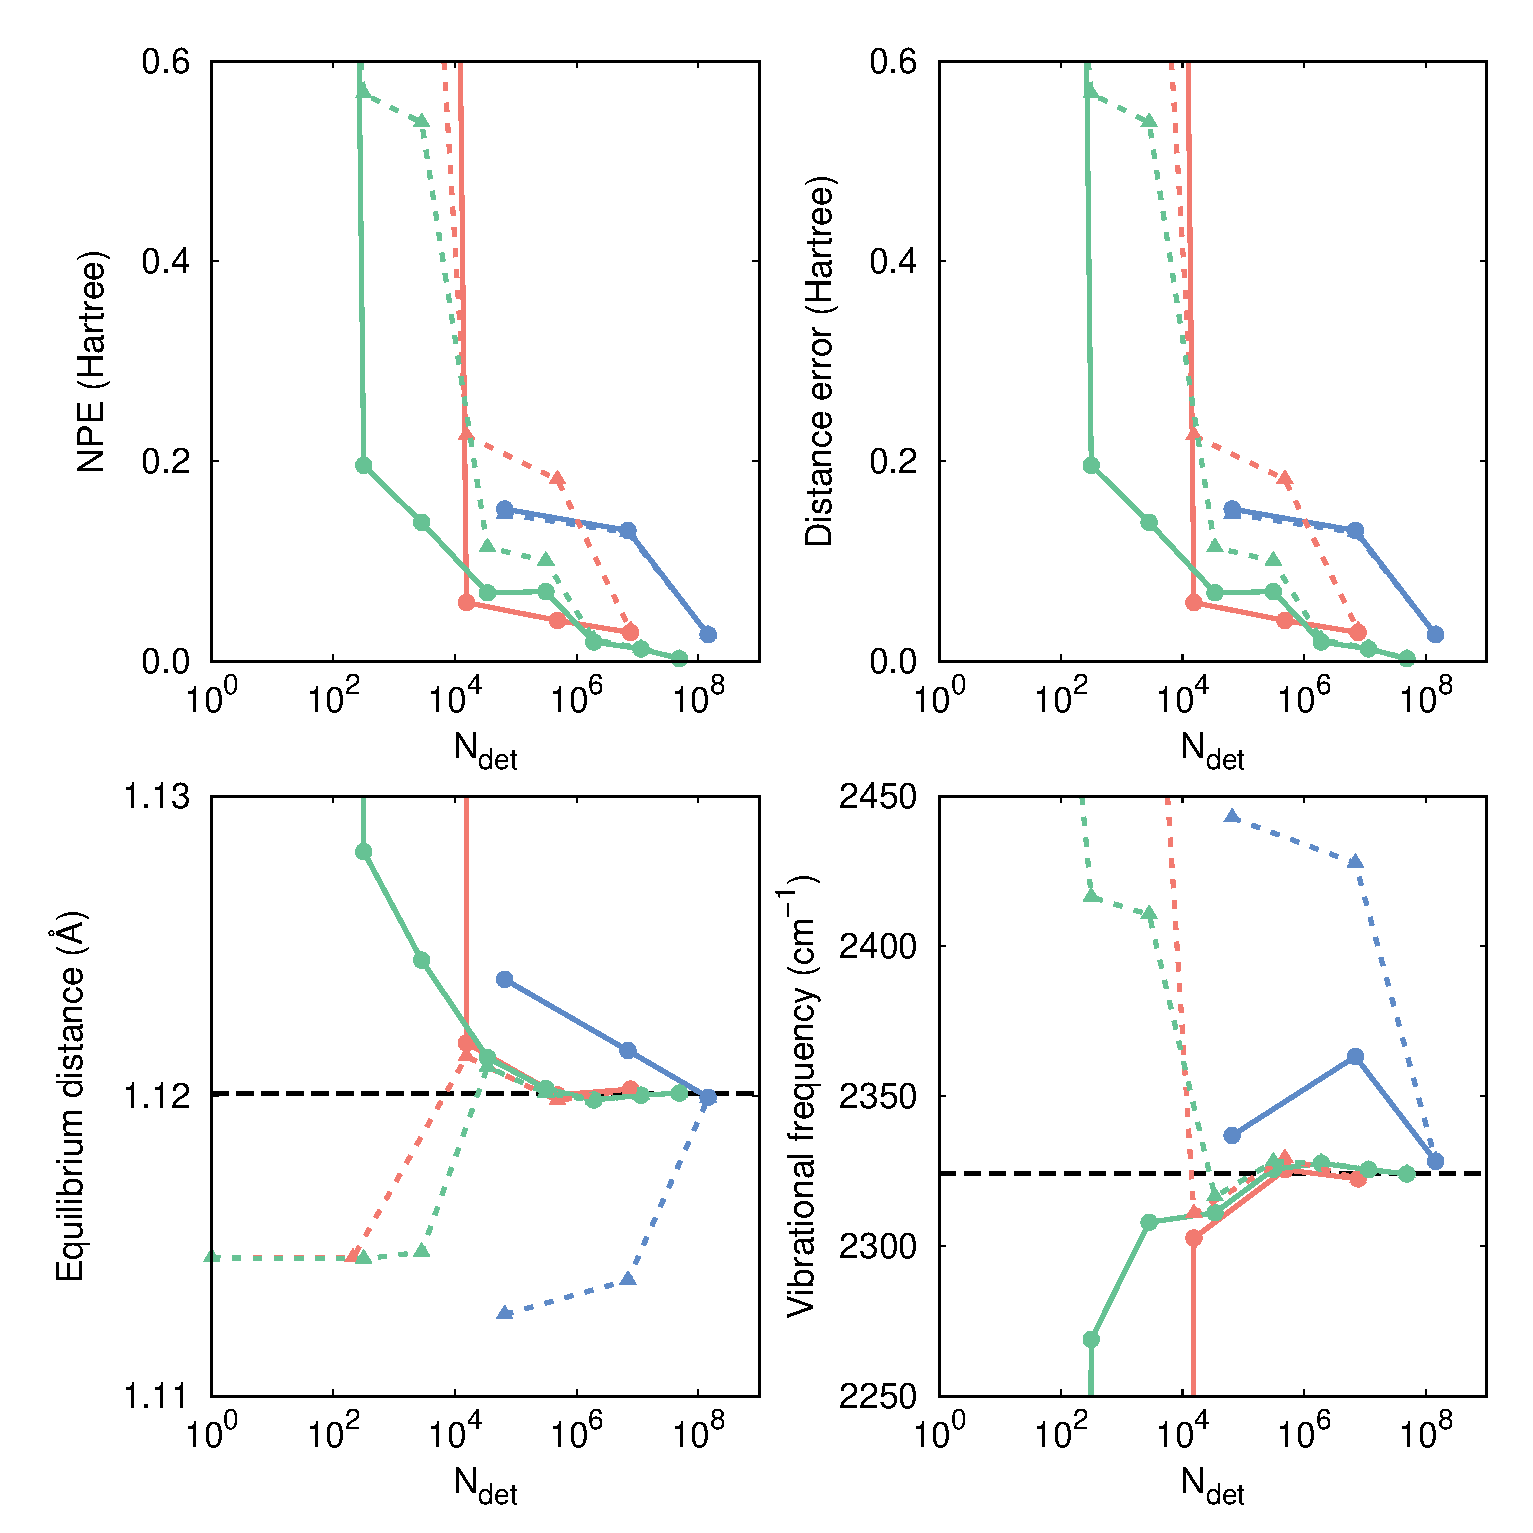
\includegraphics[width=1.0\linewidth]{plot_pt2_rpt2_N2}
\caption{
\ce{N2}
}
\label{fig:plot_pt2_rpt2_n2}
\end{figure*}
%%% %%% %%%

%%% FIG S3 %%%
\begin{figure*}%[h!]
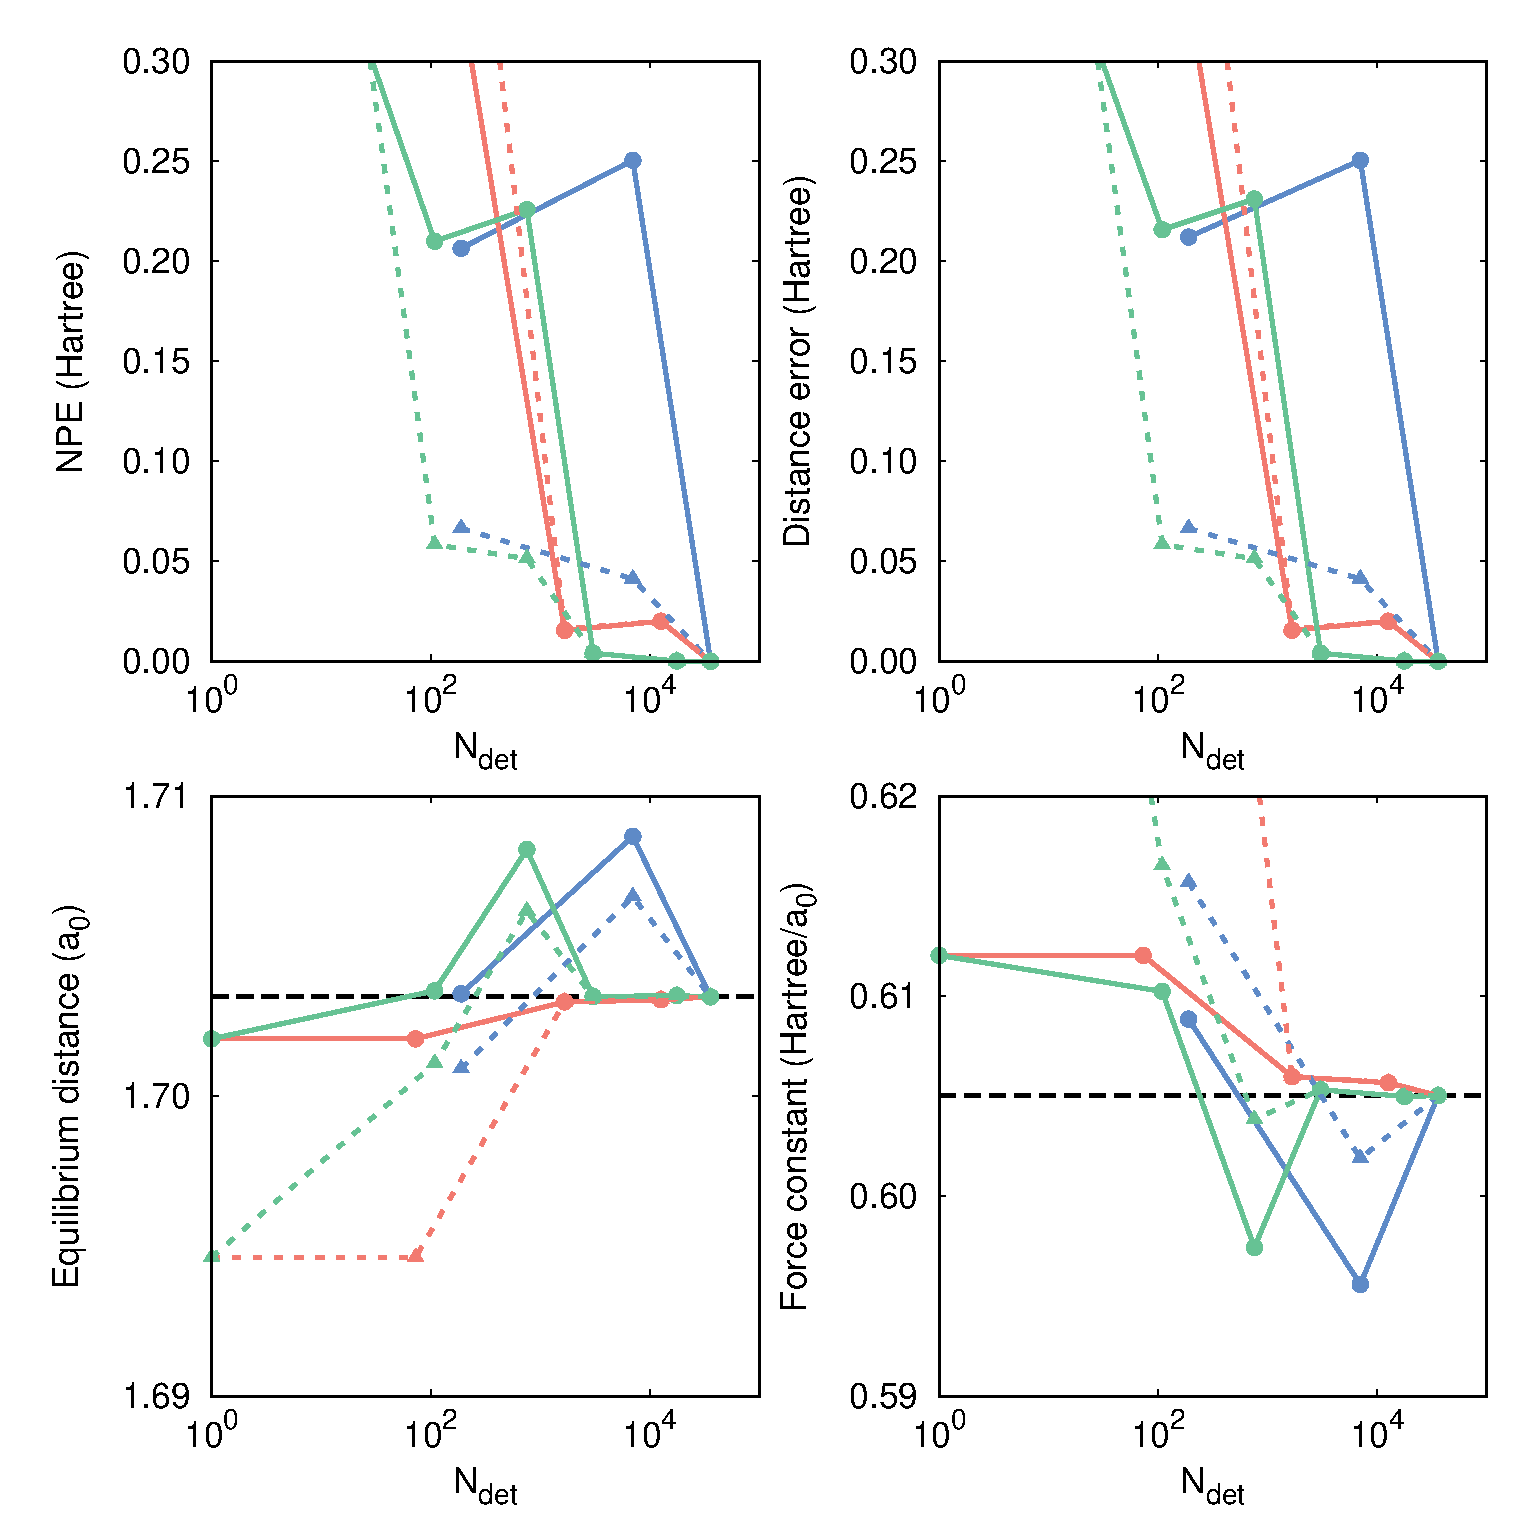
\includegraphics[width=1.0\linewidth]{plot_pt2_rpt2_H4}
\caption{
\ce{H4}
}
\label{fig:plot_pt2_rpt2_h4}
\end{figure*}
%%% %%% %%%

%%% FIG S3 %%%
\begin{figure*}%[h!]
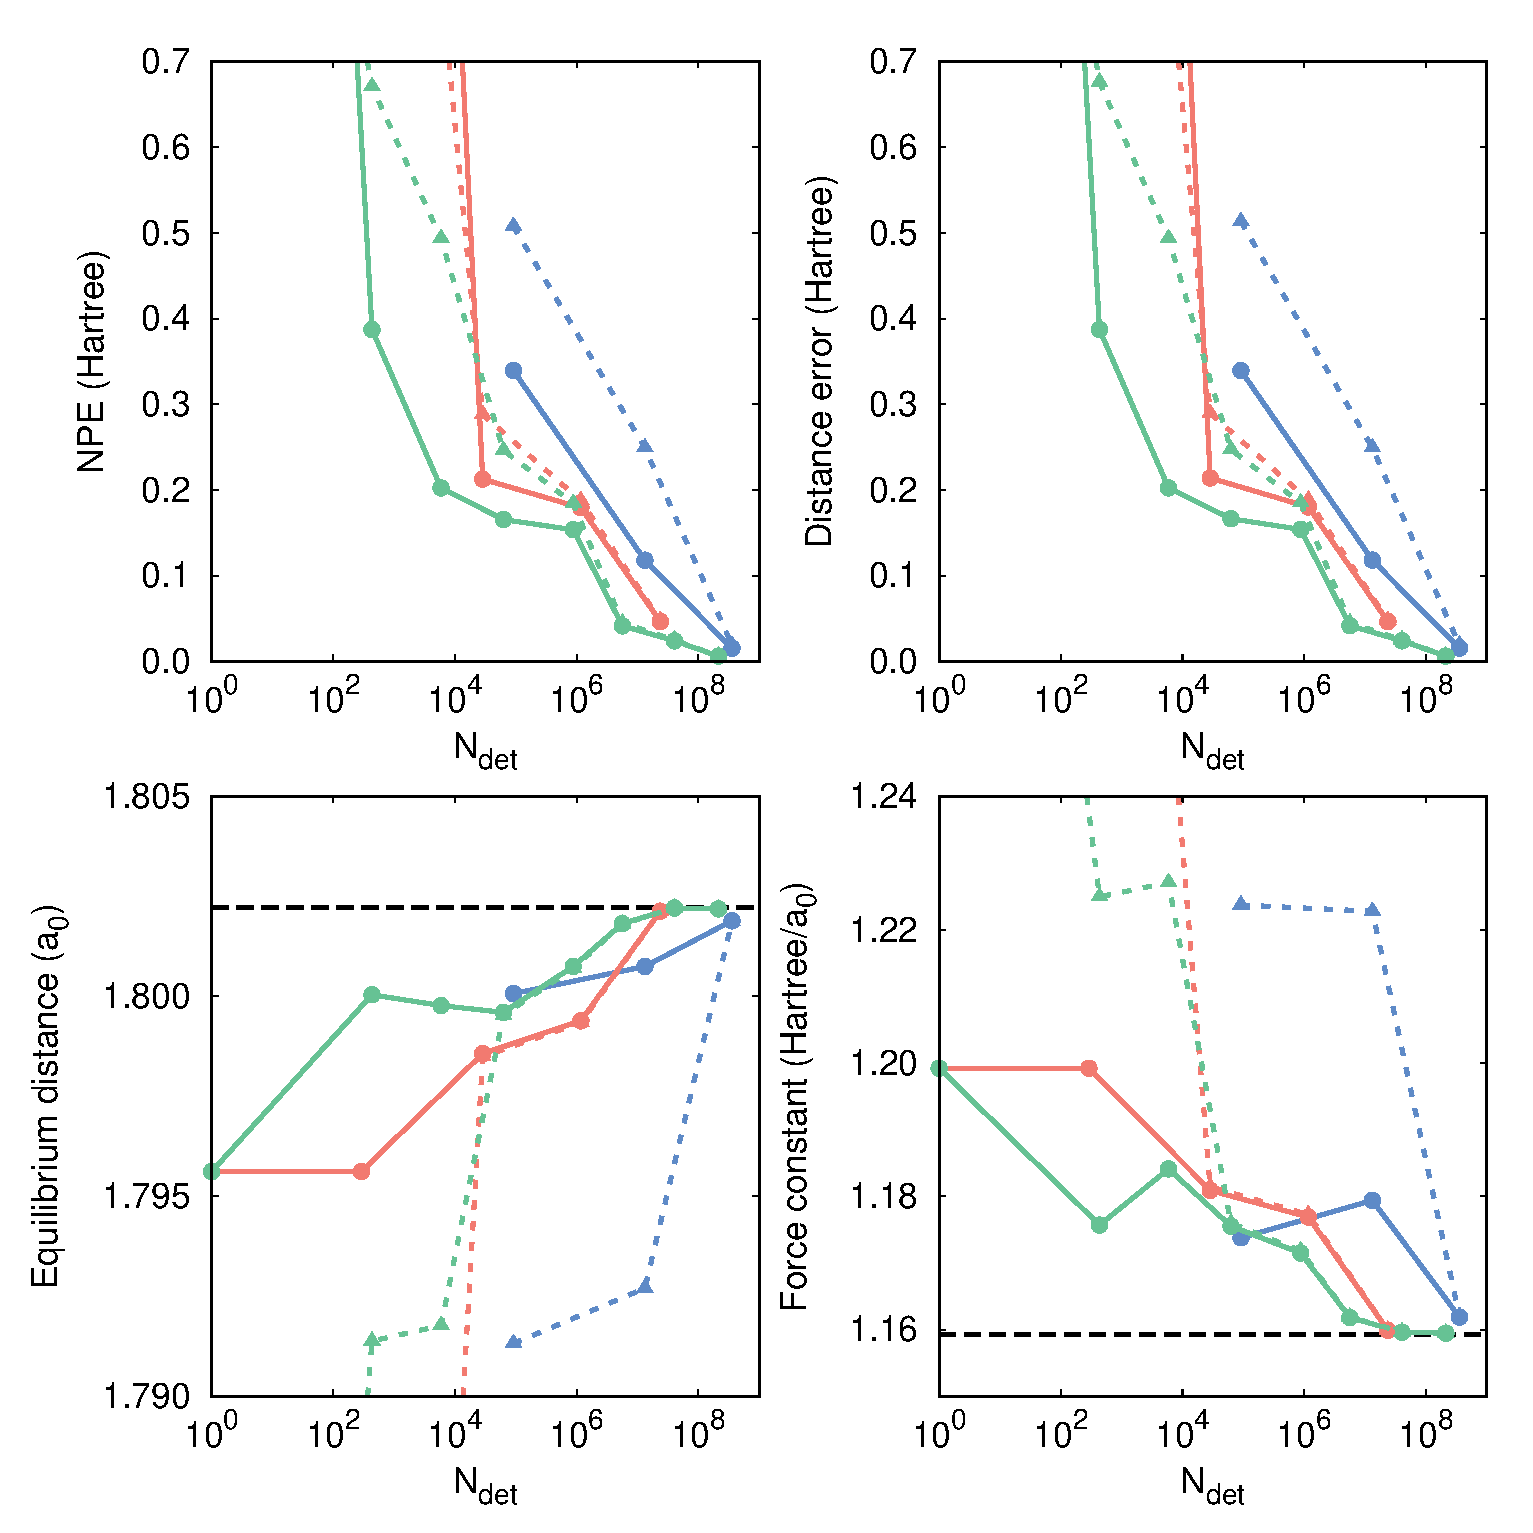
\includegraphics[width=1.0\linewidth]{plot_pt2_rpt2_H8}
\caption{
\ce{H8}
}
\label{fig:plot_pt2_rpt2_h8}
\end{figure*}
%%% %%% %%%


\clearpage

%%%%%%%%%%%%%%%%%%%%%%%%%%%%%%%%
\bibliography{manuscript}
%%%%%%%%%%%%%%%%%%%%%%%%%%%%%%%%

\end{document}
